
\section{High-Level Tasks}
\label{sec:apps}

%Detection, Recognition, xxx


%tbd: level-wise? scope \& coverage

This section reviews high-level tasks in multimedia analytics built upon deep learning framework. This survey covers various task involved in multimedia analytics, with a focus on visual data, i.e., image and video. 

Fig.~\ref{fig:overview} shows the roadmap of multimedia analytics, which focuses on analyzing multimedia data (left) from diverse perspectives (right). 

\begin{itemize}
	\item multimedia $\rightarrow$ label.
	%
	\item multimedia $\rightarrow$ location. 
	%
	\item multimedia $\rightarrow$ sentence.
	%
	\item multimedia $\rightarrow$ paragraph.
	%
	\item multimedia $\rightarrow$ image.
	%
	\item Image/Video generation (reverse mapping). Generating images given a label, paragraph texts, etc..
\end{itemize}

For example, image classification aims to translate an image to one or multiple labels, while image captioning parse an input image to a sentence. The difficulty of each task increases as the capacity of target domain grows. Moreover, the reverse mapping (from left to right) is also valid, due to recent advancement of Generative Adversarial Networks (GAN). 


\begin{figure}[t]
	\begin{center}
		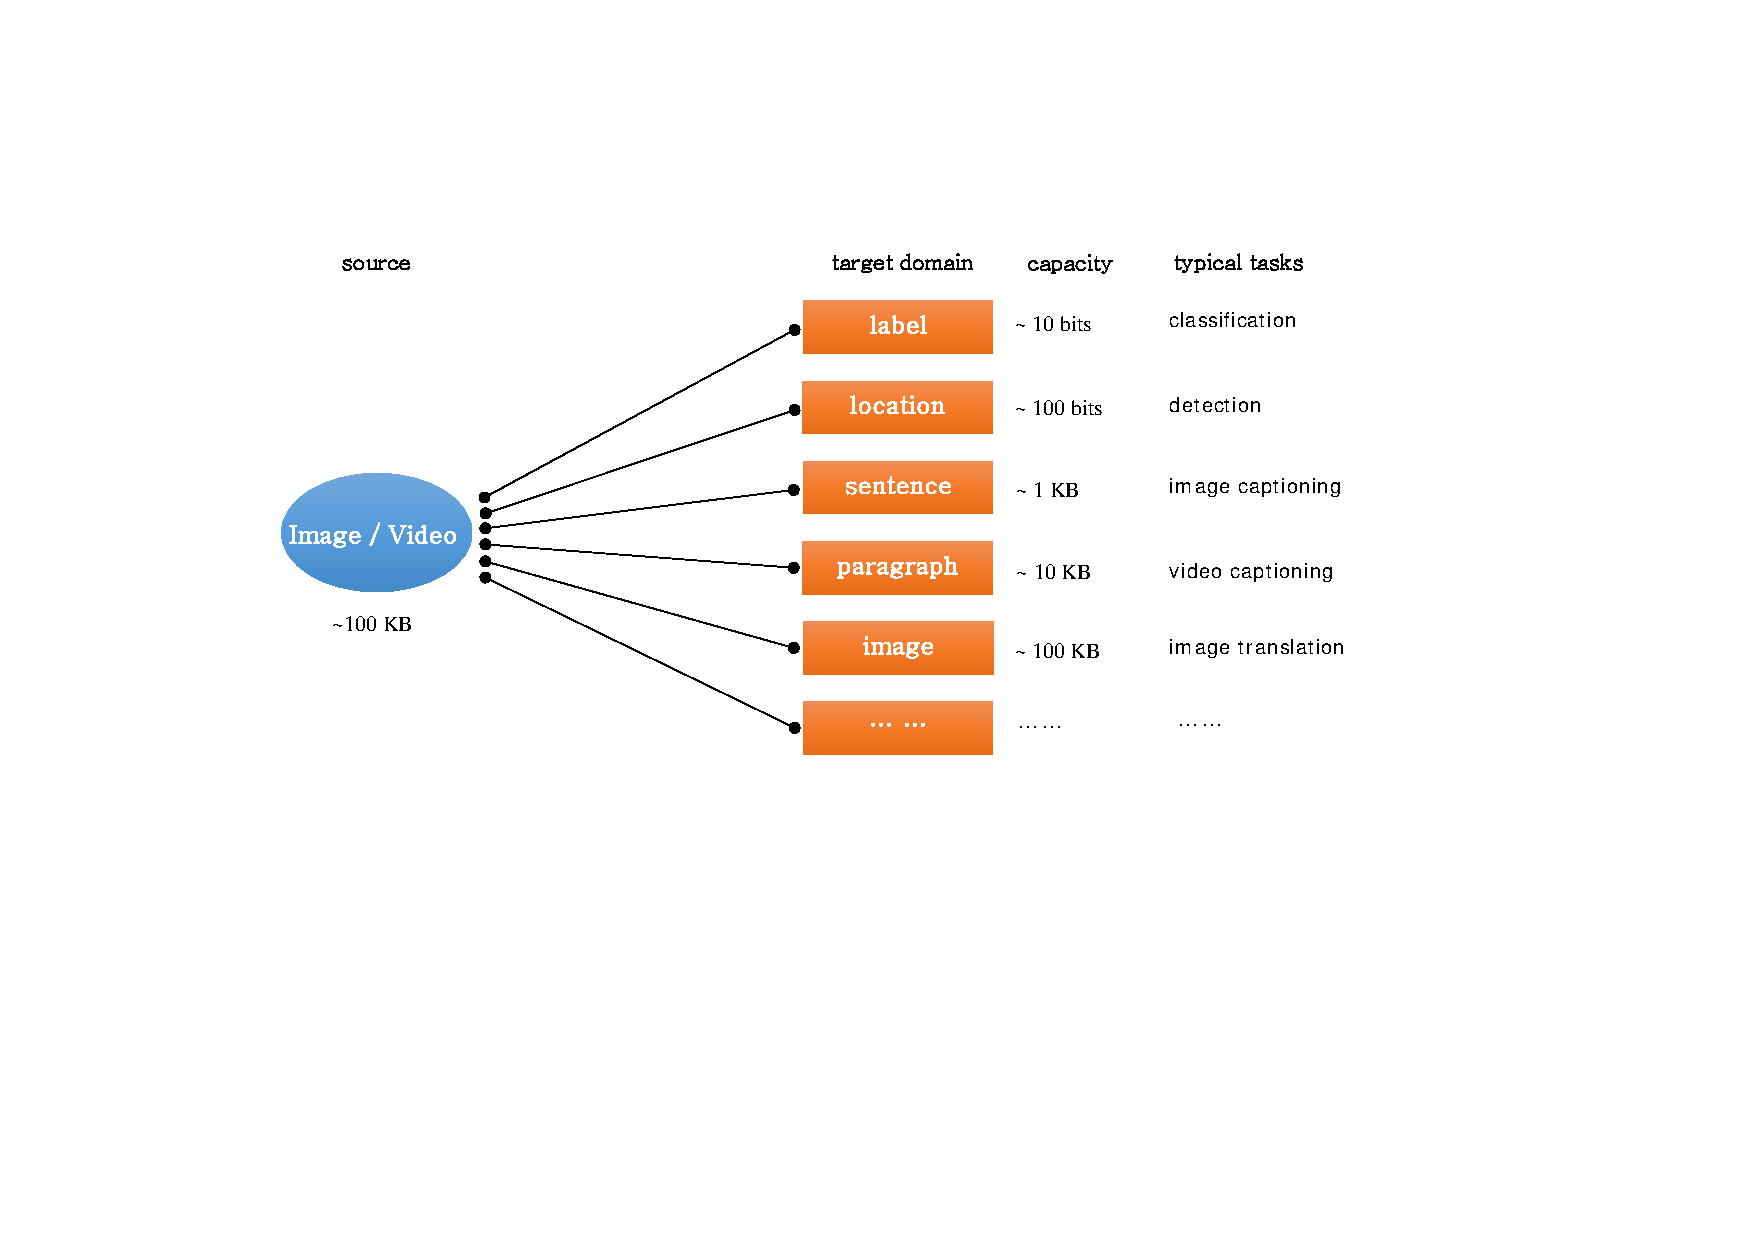
\includegraphics[width=5in]{figs/overview.pdf}
	\end{center}
	\caption{A road-map for deep learning based multimedia analytics. }
	\label{fig:overview}
\end{figure}

\subsection{Detection}

\begin{figure}[t]
	\begin{center}
		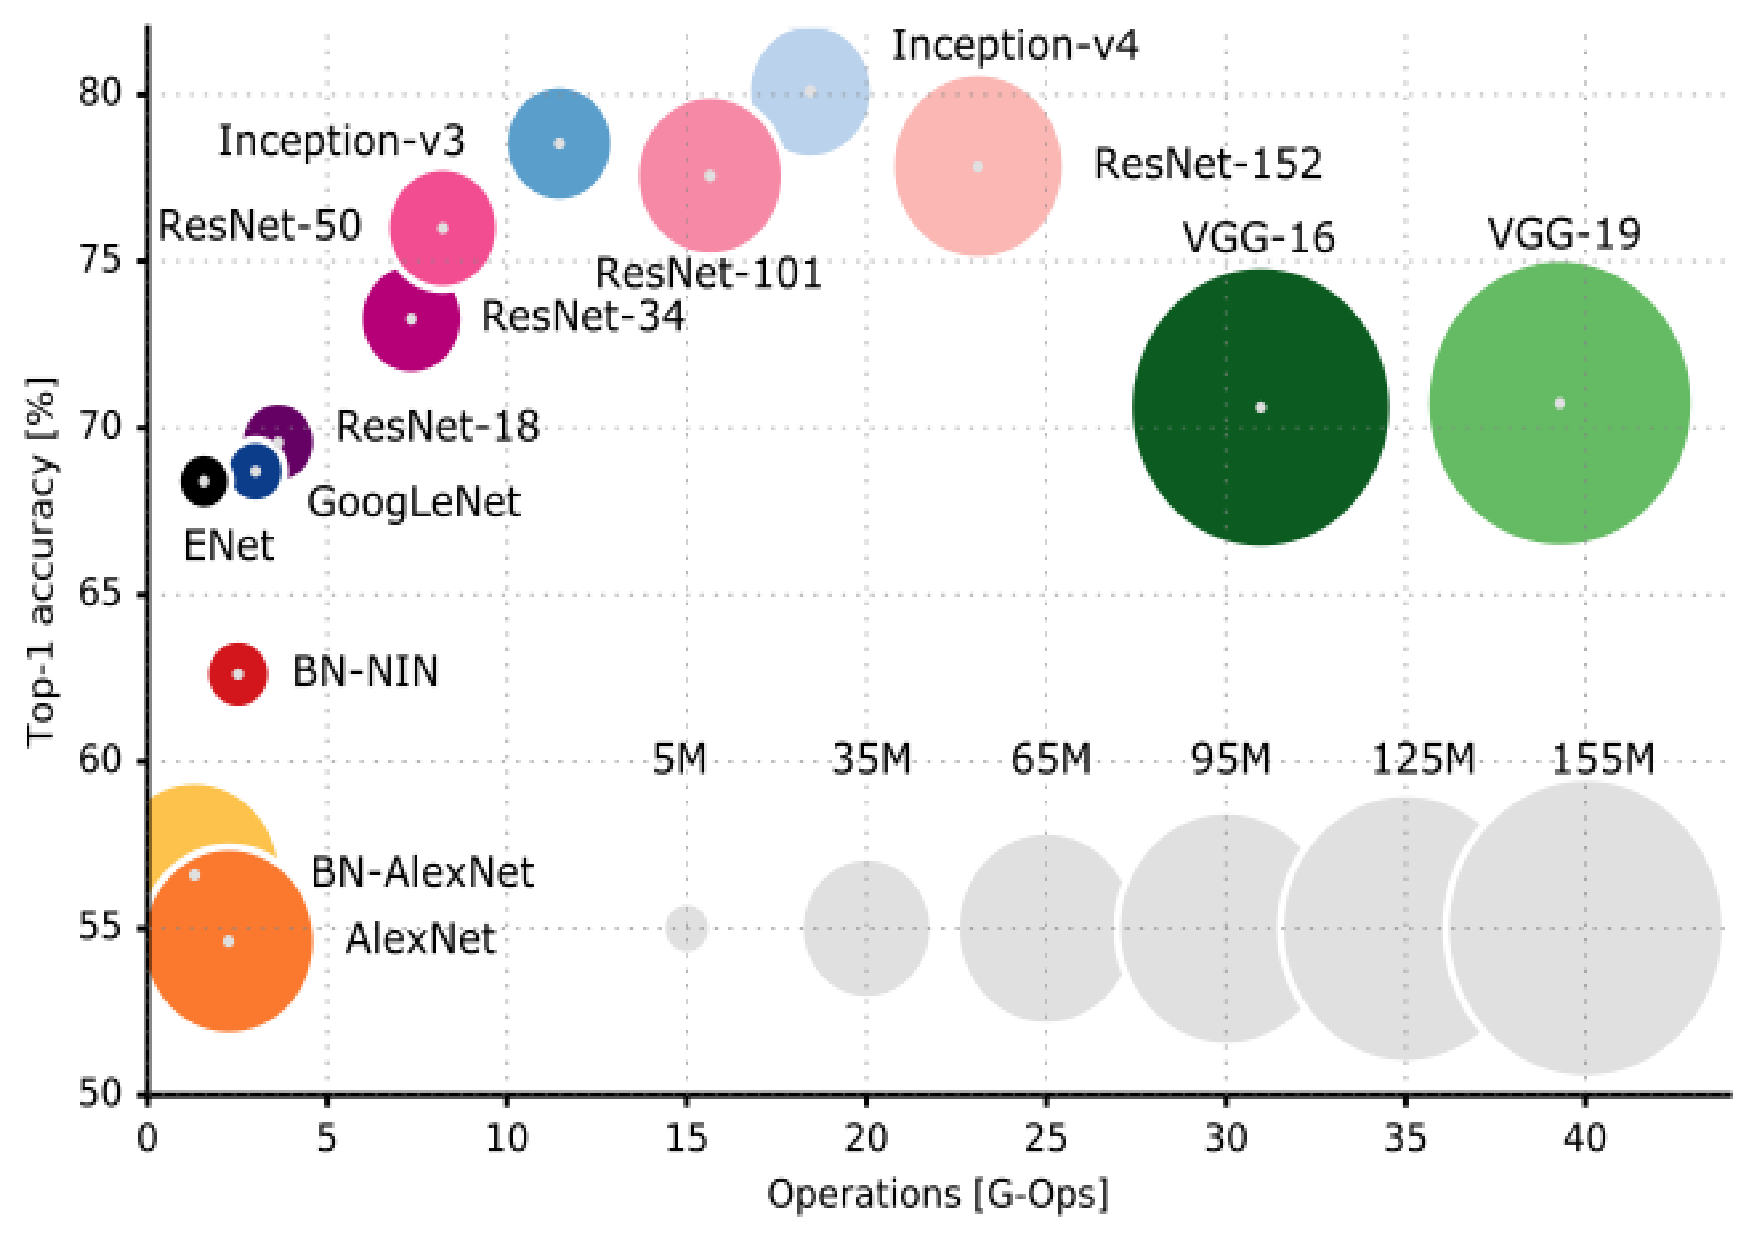
\includegraphics[width=4in]{figs/detection.pdf}
	\end{center}
	\caption{Major milestone on ILSVRC.}
	\label{fig:detection}
\end{figure}


Fig.~\ref{fig:detection} summarizes several milestones for image classification on ILSVRC dataset. 

\subsection{Localization}


\subsection{Captioning}


\subsection{Generation}









